\chapter{Ausführung}

    Dieses Kapitel beschreibt die Vorgehensweise von der ersten manuellen Analyse der Daten bis zum fertigen Produkt.
    Als Beispielprodukt für die Klassifizierung wurde eine Senseo Kaffeemaschine gewählt, da durch häufige Benutzung viele Daten erhoben werden können. 
    Außerdem wurde eine Mikrowelle als zweite Gerät mit wenigen Daten gewählt um verschiedene Parameter und Kennzahlen zu vergleichen.
    Hierbei soll die Anzahl der Daten sowie die Klassifikation von mehreren Geräten innerhalb eines Neuronalen Netzes untersucht werden.

\section{Manuelle Analyse} \label{ManuelleAnalyse}

    Zur manuellen Analyse der Daten wird das in \ref{VisualisierungWebApp} beschriebene Tool verwendet.
    Zunächst werden sehr aussagenkräftige Größen wie die Spannung oder die Frequenz der Kaffeemaschine verwendet und mit anderen aktiven Zeiträumen der Kaffeemaschine verglichen.
    Hierbei kann ein sehr spezifischer Verlauf der Spannung erkannt werden.\\ 
    Wie in Schaubild ref{fig:Spannungsverlauf} zu sehen ist, ist die Kurve zu Beginn start fallend und verbleibt dann eine gewissen Zeit auf diesem Tief. 
    nach einem längeren steigenden Abschnitt fällt die Kurve wieder bis der Zubereitungsvorgang beendet wurde und wieder steigt.\\
    \newline
    Diesem Verlauf können nach mehreren Beobachtungen bestimmte Vorgänge einer Kaffeezubereitung zugeordnet werden.
    Zu Beginn der Kaffeezubereitung wird die Kaffeemaschine manuell eingeschaltet. 
    Dies führt automatisch zum erwärmen des Brühwassers, welches dem ersten Fallen der Kurve zugeordnet werden kann. 
    Da dort viel Energie benötigt um das Wasser zu erhitzen steigt der Stromverbrauch der Kaffeemaschine stark an und somit fällt die Netzspannung stark ab.
    Die Netzspannung bleibt solange auf einem gewissen Tiefpunkt mit minmaler Netzschwankung bis das Wasser erwärmt wurde und ein weiterer manueller Schritt zum fortfahren des Prozesses notwendig ist.\\
    Nach Wahl der Tassengröße wird dann der Brühvorgang gestartet. 
    Dabei wird das erhitzte Wasser mit einem gewissen Druck durch einen Kaffeepad gepresst. 
    Da dieser Druck bei der Senseo Kaffeemaschine durch eine elektronische Pumpe erzeugt wird, sinkt demnach die Netzspannung wird ab bis der komplette Kaffee durch gelaufen ist.
    Somit kann die Zweite Tiefpunktphase dem ``Pressvorgang'' der Kaffeemaschine zugeordnet werden.\\
    \newline
    
    \begin{figure}[H]
        \centering
        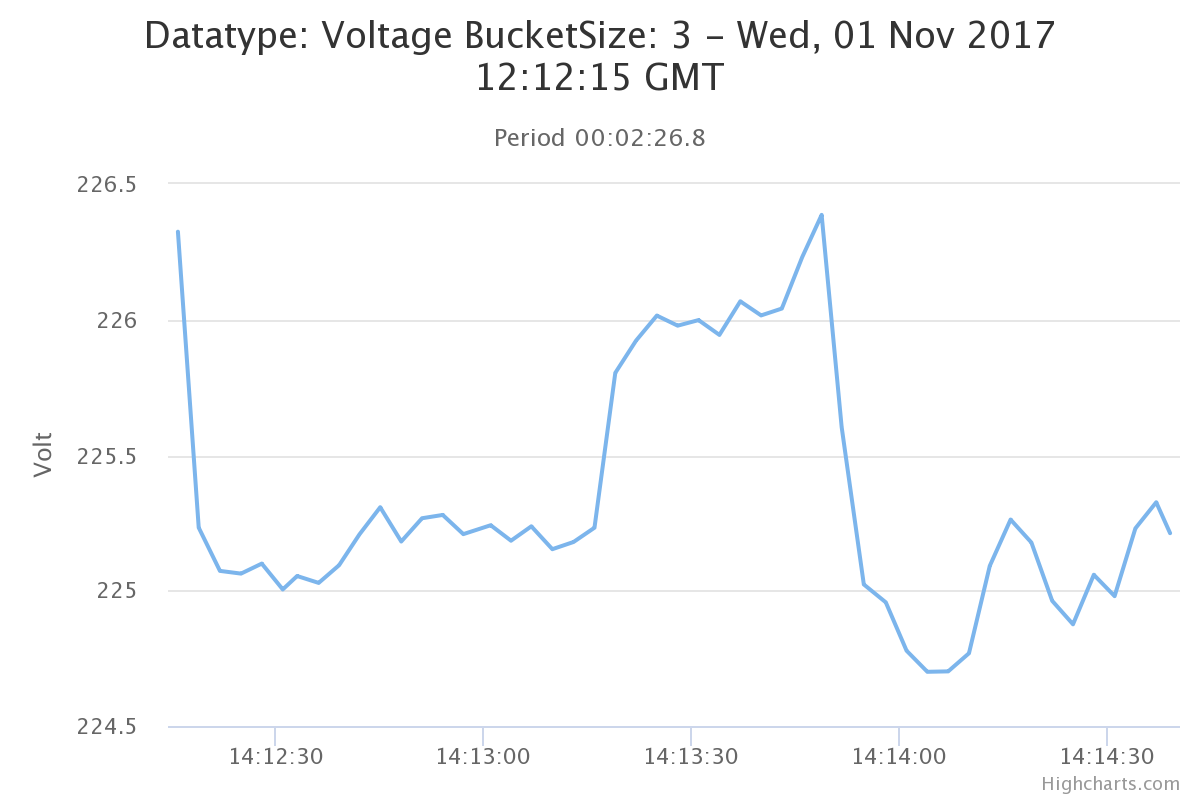
\includegraphics[width=0.8\textwidth]{SpannungsverlaufSenseo1}
        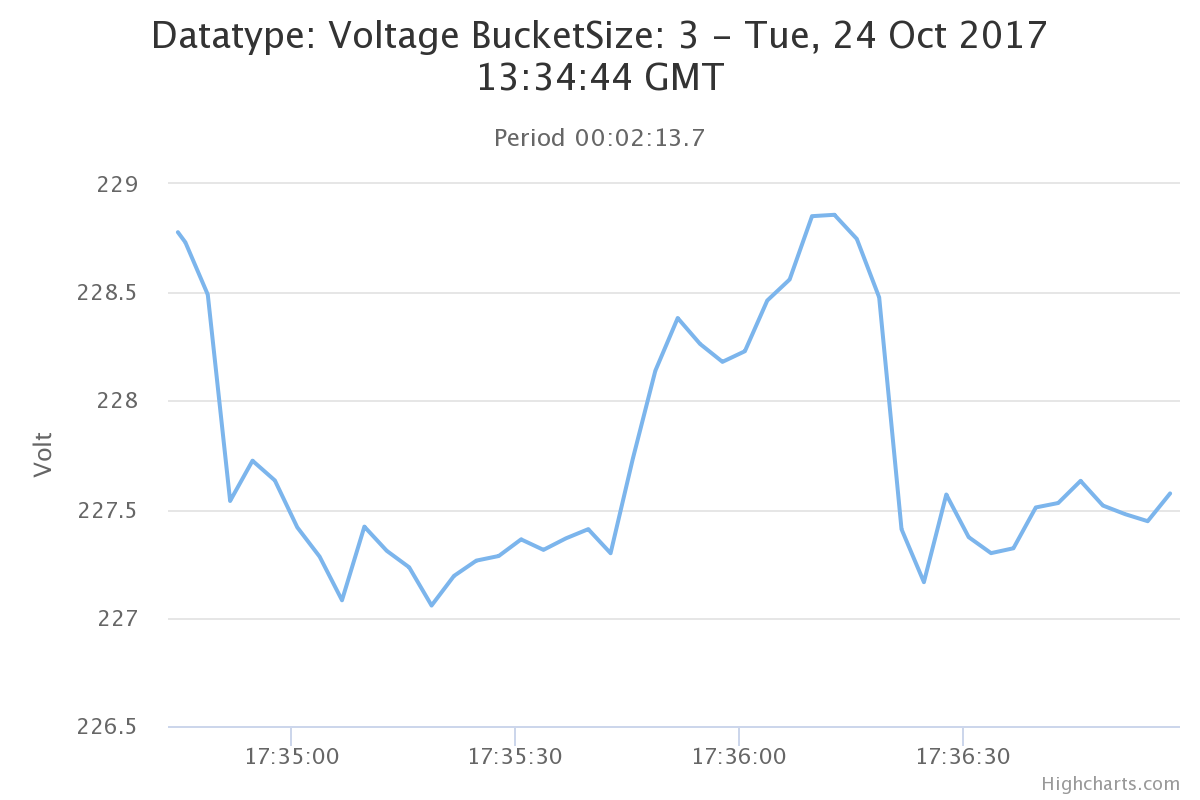
\includegraphics[width=0.8\textwidth]{SpannungsverlaufSenseo2}
        \caption{Spannungsverlauf der Senseo Kaffeemaschine mit einer Klasse von je 3 Datenpunkten zu 2 verschiedenen Zeitpunkten}
        \label{fig:SpannungsverlaufSenseo}
    \end{figure}

    \noindent
    Bei der manuellen Analyse der Mikrowelle können bei Analyse des Spannungs- oder Frequenzverlaufs leider keine hervorstechenden Merkmale oder Gemeinsamkeiten erkannt werden.
    Somit wird die Mikrowelle demnach einen anderen Einfluss auf doe Netzaktivität ausüben.
    Wie bei dem Vergleich der verschiedenen harmonischen Oberwellen zu sehen ist (siehe Schaubild \ref{fig:3OberwelleMikrowelle}), besteht eine große Ähnlichkeit der Kurven der dritten harmonischen Welle.\\
    \newline

    \begin{figure}[H]
        \centering
        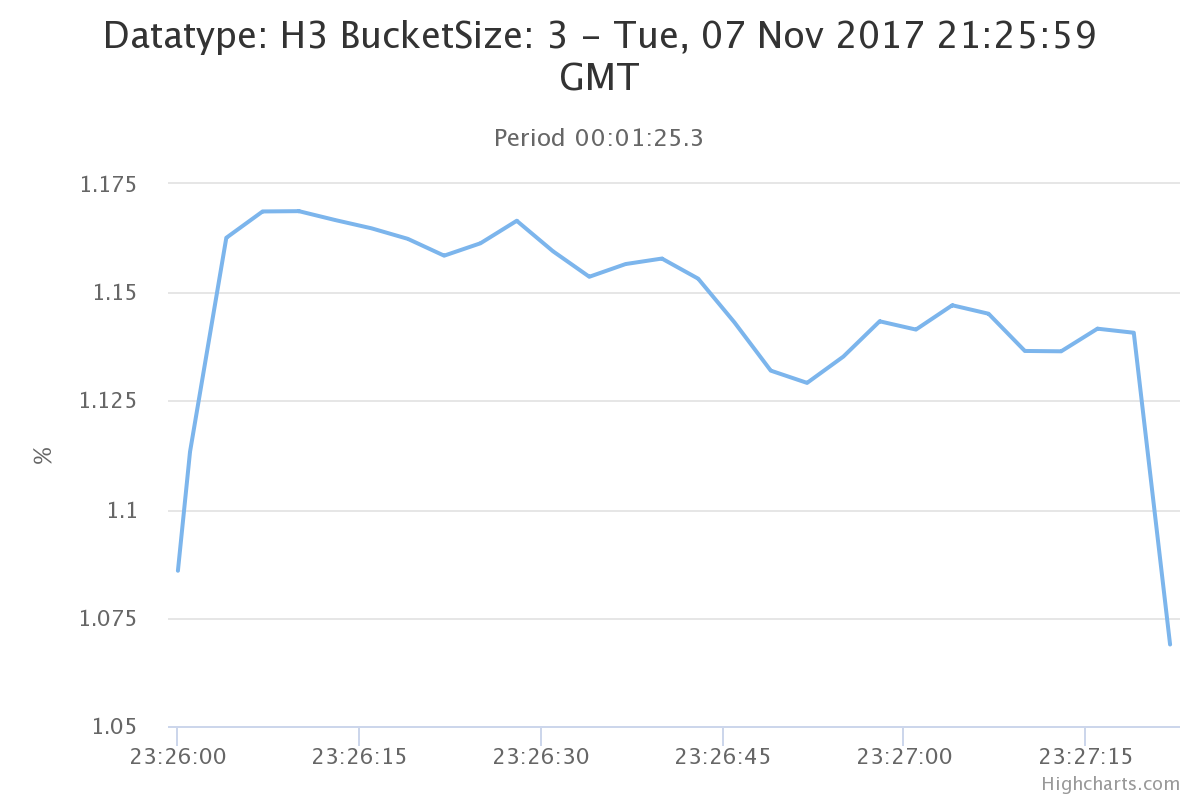
\includegraphics[width=0.8\textwidth]{3OberwelleMikrowelle1}
        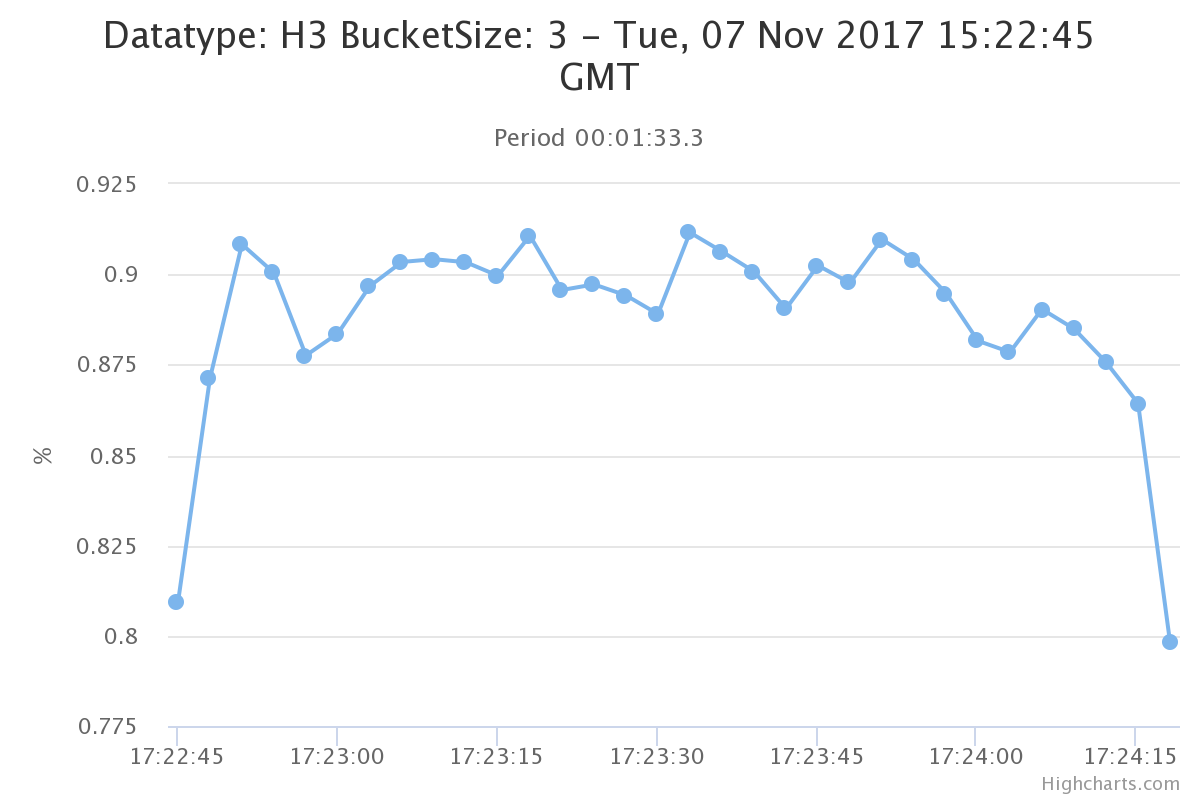
\includegraphics[width=0.8\textwidth]{3OberwelleMikrowelle2}
        \caption{Verlauf der 3. harmonischen Oberwelle einer Mikrowelle mit einer Klasse von je 3 Datenpunkten zu 2 verschiedenen Zeitpunkten}
        \label{fig:3OberwelleMikrowelle}
    \end{figure}

    \noindent
    Wie dieser Abschnitt zeigt können schon mit bloßen Auge bestimmte Auswirkungen der verschiedenen Geräte erkannt werden.
    Auch wenn einige Störungen auftreten und den Verlauf verfälschen, sollte es dennoch möglich sein diese Geräte herauszufiltern.
    Weiterführend wird dieser Prozess automatisiert und verbessert um auch trotz großer Störungen, Geräte präzise klassifizieren zu können. 

\section{Vorbereiten der Daten}\label{VorbereitenDerDaten}
    Um die Klassifizierung der Geräte auf neuronalen Netzen abzubilden müssen die vorhandenen Daten in ein geeignetes Format transformiert werden.
    Dabei gibt es verschiedene Vorraussetzungen zu beachten, sowie verschiedene Möglichkeiten die Daten zu transformieren.\\
    
    \noindent
    Bei konventionellen Neuronalen Netzen werden Eigenschaften Objekten zugewiesen, wobei alle Objekte mit denselben Eigenschaften betitelt werden.
    Ein Beispiel dafür sind Tiere, bei denen anhand von Reproduktion oder Atmung in Säugetiere, Vögel, Reptilien, etc. eingeteilt wird. 
    So können spezielle Tiere wie ein Hund in eine dieser Klassen zugewiesen werden.
    Alle klassifizierten Tiere werden hierbei dieselben Eigenschaftsklassen mit unterschiedlichen Werten zugewiesen.
    Das heißt, dass einem Hund oder einer Taube die Anzahl der Beine und die Reproduktion zugewiesen werden jedoch mit jeweils unterschiedlichen Werten.\\
    
    Durch die in Kapitel \ref{Messdaten} beschriebene Erhebung der Daten, werden die Stromdaten in einem bestimmten Format von der API bereitgestellt.
    Es werden 2 verschiedene Listen zurückgegeben wobei eine die reinen Messdaten enthält und die andere die Labels für diese Daten.\\
    Die reinen Messdaten werden zusammengetragen, indem zu den gelabelten Zeiträumen jeweils alle sekündlich gemessenen Werte des Stromnetzes als eine Matrix eingefügt werden.
    Somit ergibt sich eine drei dimensionale Matrix welche inder ersten Dimension die Zeiträume abbildet, in der zweiten Dimension die sekündliche Zeitreihe und die dritte die vorhandenen physikalischen Größen.

    \begin{lstlisting}[language=Python, caption={Datenstruktur der gelabelten Messdaten, die von der API bereit gestellt wird},label=lst:DatenstrukturGelabelteMessdaten]

[
    [
        [u, f, h3, h5, h7, h9, h11, h13, h15],
        [u, f, h3, h5, h7, h9, h11, h13, h15],
        [u, f, h3, h5, h7, h9, h11, h13, h15],
        ...
    ]
]
    \end{lstlisting}

\section{Neuronales Netz}
    Wie Abschnitt \ref{ManuelleAnalyse} zeigt ist es möglich mit herkömmlichen manuellen Methoden verschiedene Geräte innerhalb eines Verlaufs zu klassifzieren.
    Somit sollte dies auch mit maschinellem Lernen möglich sein.
    \newline

    \noindent
    Um nun die Geräte maschinell zu klassifiziren, werden drei verschiedene "`neuronale Netz"' Modelle erstellt und miteinander verglichen.
    Die drei Modelle beinhalten ein "`Recurrent Neural Network(RNN) "', ein "`Convolutional Neural Network(CNN)"' sowie eine Mischung aus diesen Ansätzen. 
    Da Neuronale Netze feste Eingabegrößen benötigen, werden die Daten wie im Abschnitt \ref{VorbereitenDerDaten} in Batches aufgeteilt.
    Um die bestmöglichste Batchgröße zu erreichen werden verschiedene Größen getestet.

    \subsubsection{CNN}
    Grundlegend besteht das "`Convolutional Neural Network(CNN)"' aus einem "`Input Layer"', drei "`Convolutional Layers"', einem "`Dropout Layer"' sowie einem "`Output Layer"'.
    \newline

    \noindent
    Das "`Input Layer"' ist der Eingang zum neuronalen Netz, welcher die Rohdaten annimmt und an das eigentliche Netz weiterleitet. 
    Es nimmt einen Eingabe-Tensor (Matrix innerhalb eines neuronalen Netzes), welcher an die Batchgröße angepasst wird.
    \newline

    \noindent
    Die Eingabe wird dann weitergeleitet an die drei "`Convolutional Layers"', welche mit unterschiedlicher "`Hidden Layer"'-Größe initialisiert werden.
    Wobei die "`Hidden Layer"' größer werden je näher sie topologisch an dem "`Output Layer"' liegen.
    \newline

    \noindent
    Das "`Dropout Layer"' wird eingefügt um die Tensordimension zu verkleinern und somit das Ergebnis zu Generalisieren und Overfitting zu vermeiden.
    \newline

    \noindent
    Das "`Output Layer"' wandelt nun die Erkenntnisse der vorherigen Schichten in ein lesbares Fomat um. 
    Hierzu wird ein "`Dense Layer"', welcher ein eindimensionaler Tensor mit einem Feld pro klassifizierbaren Objekt. 
    Dies bedeutet, dass dieser Tensor bei einem Klassifizierung von zwei Geräten ein Array mit der Größe 2 ist. 
    \newline

    \noindent
    
    
    \begin{figure}[H]
        \centering
        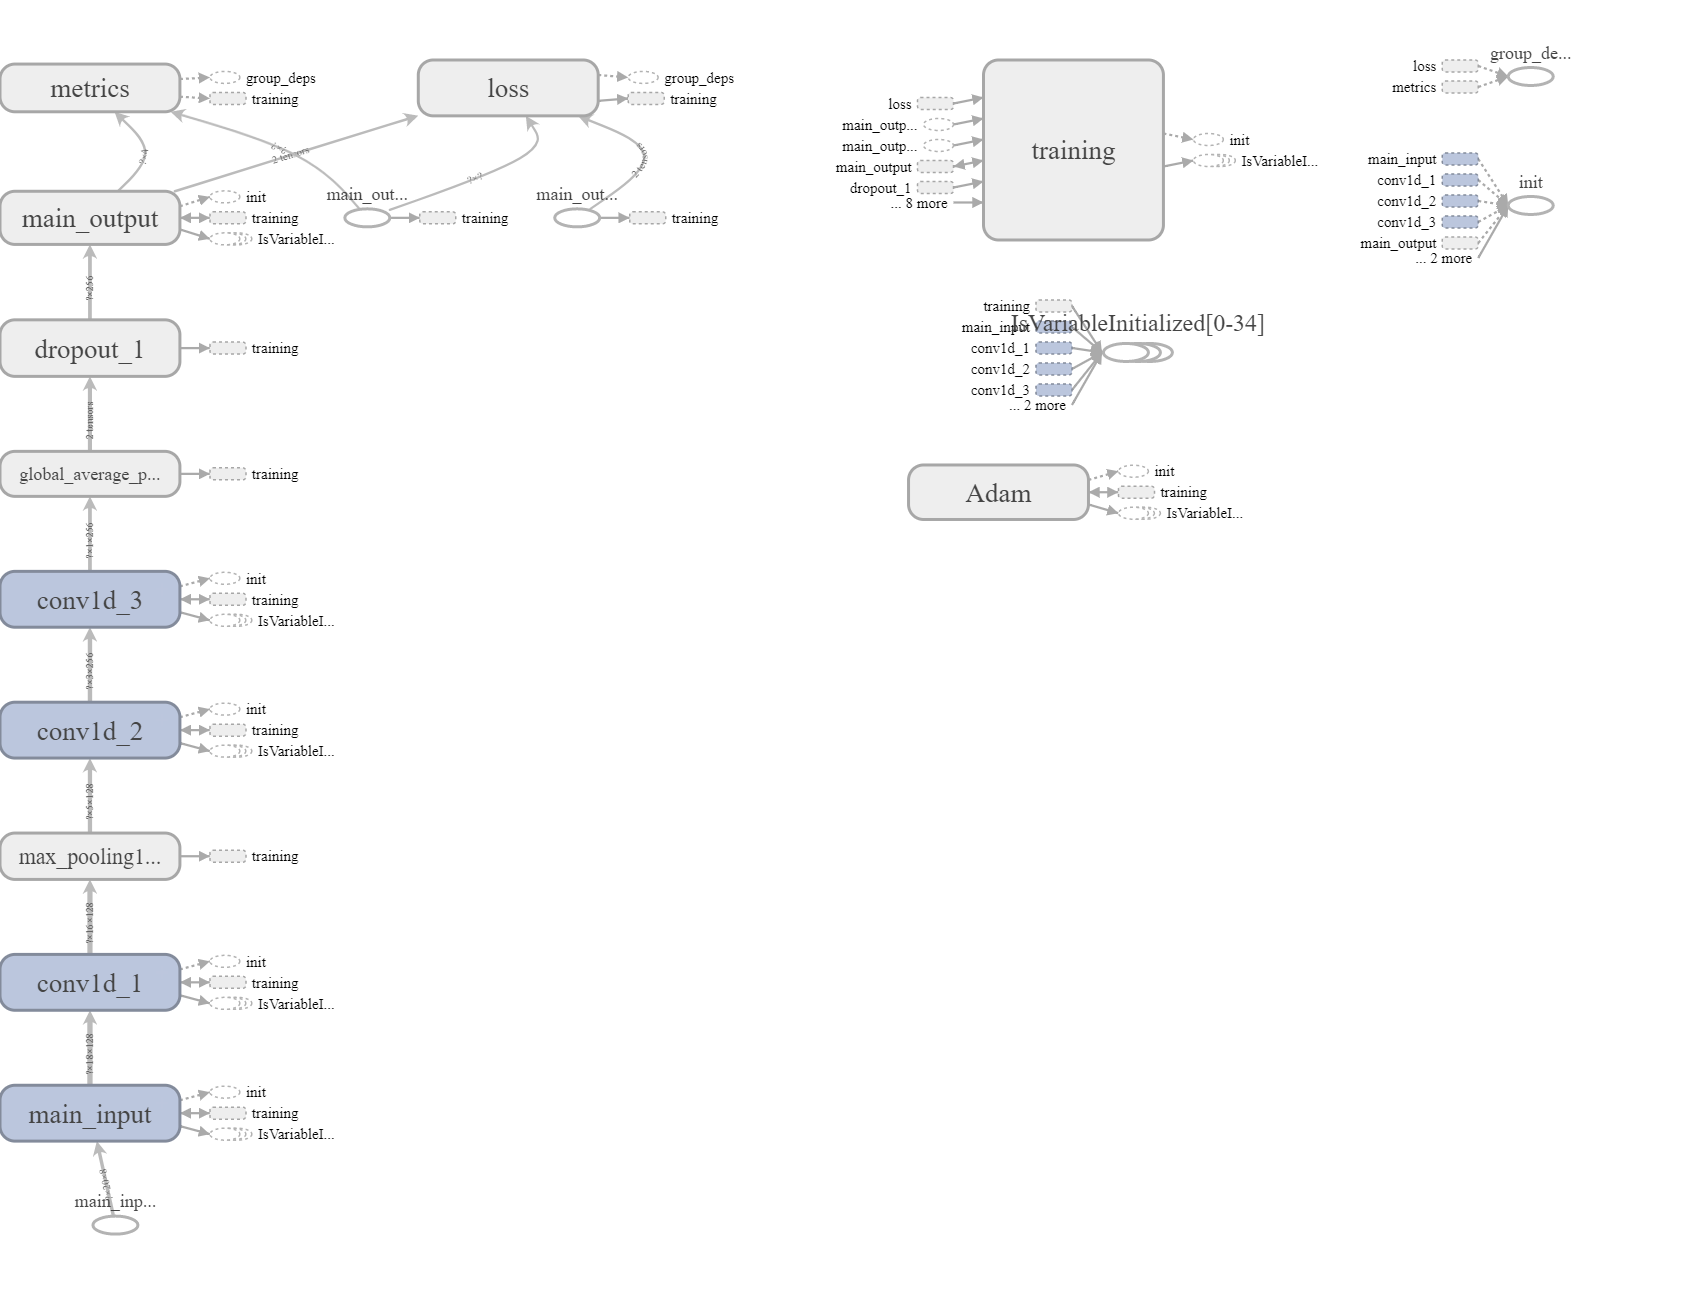
\includegraphics[width=\textwidth]{CNN_Model}
        \caption{Convolutional Neural Network}
        \label{fig:CNN_MODEL}
    \end{figure}



    
    % batches von 20 / 30 / 60
    % überlappende batches
    % 1 batch von 20 Datenpunkten pro sekunde --> mehr daten und höhere genauigkeit beim späteren klassifizieren
    % Untransformierte Daten
    % Ableitungen da Verlauf bzw. Kurve entscheidend und nicht rein Werte wie bei Bildern
    % Normalisieren auf Werte zwischen 0 und 1 um Matrizen besser auswerten zu können


\section{Trainingsprozess}

\section{Auswertung der Ergebnisse}
    % verschiedene Batch größen vergleichen
    % verschiedene neuronale Netze vergleichen CNN, RNN, CNN + RNN
    % vllt. verschiedene Aktivierungsfunktionnen Sigmoid / Cross-Entropie / Binary Cross-Entropie
